\documentclass[11pt,a4paper]{article}

% ---------- arxiv-style preamble ----------
\usepackage[margin=1in]{geometry}
\usepackage{amsmath,amssymb,amsthm}
\usepackage{graphicx}
\usepackage{longtable}
\usepackage{booktabs}
\usepackage{siunitx}
\usepackage{hyperref}
\usepackage{xcolor}
\usepackage[numbers,sort&compress]{natbib}
\usepackage{tikz}
\usetikzlibrary{positioning,arrows.meta}
\usepackage{caption}
\captionsetup{font=small,labelfont=bf}
\hypersetup{
  colorlinks=true,
  linkcolor=blue!50!black,
  citecolor=blue!50!black,
  urlcolor=blue!50!black
}

\newcommand{\sig}{\sigma}
\newcommand{\formal}{\textcolor{blue!60!black}{$\blacklozenge$}}
\newcommand{\falsi}{\textcolor{red!70!black}{$\blacksquare$}}
\theoremstyle{plain}
\newtheorem{theorem}{Theorem}
\newtheorem{lemma}{Lemma}
\newtheorem{corollary}{Corollary}
\theoremstyle{definition}
\newtheorem{claim}{Claim}

\title{
  \textbf{The \texorpdfstring{$\omega$}{omega}-Zero-Density Theorem}\\[4pt]
  \large The Dedekind discrepancy \texorpdfstring{$D(n)=\sig(n)\phi(n)-n\tau(n)$}{D(n)=sigma phi - n tau}
  vanishes at exactly \texorpdfstring{$n\in\{1,6\}$}{n in \{1,6\}}, and nowhere else
}

\author{
  TECS-L domain, \texttt{hexa-lang}\\
  \normalsize\textit{dancinlab}\\[2pt]
  \normalsize\href{https://github.com/dancinlab/hexa-lang}{\texttt{github.com/dancinlab/hexa-lang}}
}

\date{\today}

\begin{document}

\maketitle

% =========================================================================
\begin{abstract}
Define the \emph{Dedekind discrepancy} of a positive integer $n$ as
\[
  D(n) \;=\; \sig(n)\,\phi(n) \;-\; n\,\tau(n),
\]
where $\sig$ is the sum-of-divisors function, $\phi$ the Euler totient, and
$\tau$ the divisor count. We prove that the zero-locus of $D$ is the
\emph{exact two-element set} $\{1,6\}$: $D(n)=0 \iff n\in\{1,6\}$, with
$D(n)\neq 0$ for every other $n$. Because the zero set is finite, the natural
density of $\{n : D(n)=0\}$ is $0$ --- hence the name. The proof reduces $D=0$
to a multiplicative product condition $\prod_{p^a\|n} g(p,a)=1$ with
$g(p,a)=(p^{a+1}-1)/(p(a+1))$, and shows that the \emph{only} sub-unity factor
on the prime-power locus is $g(2,1)=\tfrac34$, cancelled \emph{uniquely} by
$g(3,1)=\tfrac43$ --- pinning the sole non-trivial zero to $n=2\cdot3=6$, the
first perfect number. We pre-register a single falsifier
(\textsc{f-omega-zero-density}: \emph{any} $n\notin\{1,6\}$ with $D(n)=0$) and
discharge it two ways: (i) a machine-checked sweep that recomputes $\sig,\phi,
\tau$ closed-form for an $\omega$-stratified sample spanning $\omega(n)\in[0,6]$
--- primes, prime powers, both first perfect numbers, and the primorials
$2\#,\dots,13\#$ --- every value of which is verified
\formal\,\textsc{formal} under the \texttt{hexa verify} discipline; and (ii)
the closed-form product argument above, which closes the infinite tail. The
headline finding unifies the F14--F18 TECS-L cycle: the folklore that ``$6$ is
special'' is here made into a sharp, machine-audited \emph{global} statement
rather than a local coincidence at one or two test points. No claim in this
paper is graded by a language model; every verdict is the verbatim standard
output of a deterministic recomputation.
\end{abstract}

% =========================================================================
\section{Introduction}
\label{sec:intro}

The integer $6$ is the first \emph{perfect} number, $\sig(6)=12=2\cdot6$, and
it accrues a reputation for being arithmetically exceptional. Such folklore is
rarely sharpened into a statement that is simultaneously (a) global --- a claim
about \emph{all} $n$, not a coincidence checked at a handful of points --- and
(b) machine-auditable end to end. This paper does both for one specific
discrepancy functional.

Let $\sig(n)=\sum_{d\mid n}d$, let $\phi(n)=\#\{1\le k\le n:\gcd(k,n)=1\}$ be
the Euler totient, and let $\tau(n)=\#\{d:d\mid n\}$ be the divisor count.
Define the \emph{Dedekind discrepancy}
\begin{equation}
  D(n) \;=\; \sig(n)\,\phi(n) \;-\; n\,\tau(n).
  \label{eq:D}
\end{equation}
A direct computation gives $D(1)=1\cdot1-1\cdot1=0$ and
$D(6)=12\cdot2-6\cdot4=24-24=0$. The question this paper settles is whether
\emph{any other} $n$ shares this property.

\paragraph{Main result.}
\begin{theorem}[$\omega$-zero-density]
\label{thm:main}
For every positive integer $n$,
\[
  D(n) = 0 \quad\Longleftrightarrow\quad n \in \{1,6\}.
\]
Consequently $\#\{n\le N : D(n)=0\}=2$ for all $N\ge6$, so the zero set has
natural density $0$.
\end{theorem}

\noindent The name reflects the corollary: the zero set, being finite, is
density-zero, and the proof is organised by $\omega(n)$, the number of distinct
prime factors. The case analysis is $\omega=0$ (trivial), $\omega=1$ (no zero),
$\omega=2$ (exactly $n=6$), and $\omega\ge3$ (no zero) --- the last being the
quantitative heart, where every additional distinct prime drives the governing
product strictly above unity.

\paragraph{Relation to prior TECS-L work.}
A previous note in this line established that, \emph{over the finite window}
$n\in[1,100]$, the zero set of $D$ is $\{1,6\}$, framed as one of five
``identity-locus'' coincidences at $n=6$ that each fail at the second perfect
number $28$~\citep{tecsLn6}. That treatment is local: it exhibits two test
points and a finite sweep. The present paper supersedes it with a
\emph{global} theorem and a closed-form proof that closes the infinite tail
$n>100$, and reframes the result as a density statement organised by
$\omega(n)$. The F14--F18 TECS-L sweep cycle, which independently re-confirmed
$D\neq0$ across $\omega(n)\in[3,10]$ samples~\citep{tecsLf14}, is here unified
under a single inequality.

% =========================================================================
\section{Background}
\label{sec:background}

All three functions in~\eqref{eq:D} are multiplicative: for coprime $m,n$,
$f(mn)=f(m)f(n)$ with $f\in\{\sig,\phi,\tau\}$, and likewise $n\mapsto n$ is
completely multiplicative. The product/quotient of multiplicative functions is
multiplicative, so the \emph{ratio}
\begin{equation}
  R(n) \;:=\; \frac{\sig(n)\,\phi(n)}{n\,\tau(n)}
  \label{eq:R}
\end{equation}
is multiplicative, and $D(n)=0 \iff R(n)=1$. The proof works entirely with $R$,
evaluated on prime powers and recombined multiplicatively. We recall the
standard prime-power formulas
\[
  \sig(p^a)=\frac{p^{a+1}-1}{p-1},\qquad
  \phi(p^a)=p^{a-1}(p-1),\qquad
  \tau(p^a)=a+1 .
\]

% =========================================================================
\section{Method: the verification discipline}
\label{sec:method}

Every numeric claim is evaluated by \texttt{hexa verify --expr <fn> <args>
<expected>}, a closed-form integer recomputation built into the \texttt{hexa}
compiler. The evaluator emits one of six tiers; only three are terminal and
admissible as a paper-section claim:
\begin{description}\itemsep0.2em
\item[\formal\,\textsc{formal}] a closed-form/symbolic identity reproduced exactly (deterministic).
\item[\textcolor{green!50!black}{$\bullet$}\,\textsc{numerical}] a libm/Newton numerical recompute matching to $\varepsilon=10^{-9}$.
\item[\falsi\,\textsc{falsified}] the recomputation deterministically \emph{disagrees} with the claim --- a closed negative.
\end{description}
Citation-only, deferred, and speculation-fenced tiers are \emph{not} admissible
and are reported as residuals in \textsection\ref{sec:limits}. The raw standard
output of every run is persisted verbatim under
\texttt{.verdicts/paper-omega-zero-density/} and indexed in
\texttt{CLAIMS.tape}; nothing in this paper is graded by a language model.

\paragraph{Composite values.} The discrepancy $D(n)$ has no single built-in
evaluator; we verify each factor ($\sig$, $\phi$, $\tau$) closed-form via three
independent \texttt{hexa verify --expr} calls, then form $D(n)$ by exact
integer arithmetic on the verified values. This is faithful because each factor
is an exact integer, so the product and difference are exact --- no tolerance,
no estimation, no floating point enters any \formal-tier claim here.

\paragraph{Worked example.} To anchor $D(6)=0$ one runs three calls:
\texttt{hexa verify --expr sigma 6 12}, \texttt{--expr phi 6 2},
\texttt{--expr tau 6 4}. The evaluator recomputes
$\sum_{d\mid6}d=1+2+3+6=12$, $\#\{k<6:\gcd(k,6)=1\}=2$, and $\#\{d\mid6\}=4$,
each emitting the \textsc{formal} tier; the discrepancy
$12\cdot2-6\cdot4=0$ follows by exact integer arithmetic. The pre-registered
falsifier at the second perfect number $n=28$ is the same call shape; its
closed negative $D(28)=56\cdot12-28\cdot6=672-168=504\neq0$ is read off exact
integers.

\paragraph{The closed-form half.} The infinite tail $n>30030$ cannot be swept;
it is closed by the algebraic argument of \textsection\ref{sec:proof}, whose
single inequalities ($g(2,1)<1$, all other $g>1$) are themselves exact rational
comparisons. The machine sweep and the proof are complementary: the sweep
spot-checks the proof's predictions at concrete $\omega$-stratified points; the
proof generalises the sweep to all $n$.

% =========================================================================
\section{The reduction to a product condition}
\label{sec:reduction}

\begin{lemma}[prime-power ratio]
\label{lem:g}
For a prime $p$ and exponent $a\ge1$,
\[
  R(p^a)\;=\;\frac{\sig(p^a)\phi(p^a)}{p^a\,\tau(p^a)}
  \;=\;\frac{p^{a+1}-1}{p\,(a+1)} \;=:\; g(p,a).
\]
\end{lemma}
\begin{proof}
Substituting the prime-power formulas of \textsection\ref{sec:background},
\[
  R(p^a)=\frac{\dfrac{p^{a+1}-1}{p-1}\cdot p^{a-1}(p-1)}{p^a(a+1)}
        =\frac{(p^{a+1}-1)\,p^{a-1}}{p^a(a+1)}
        =\frac{p^{a+1}-1}{p\,(a+1)} . \qedhere
\]
\end{proof}

\noindent By multiplicativity of $R$ and Lemma~\ref{lem:g},
\begin{equation}
  D(n)=0 \iff R(n)=1 \iff \prod_{p^a\,\|\,n} g(p,a)=1 .
  \label{eq:prodcond}
\end{equation}
The entire theorem is now a statement about which products of the rationals
$g(p,a)$ equal $1$.

% =========================================================================
\section{Proof of the theorem}
\label{sec:proof}

\begin{lemma}[sign of the factors]
\label{lem:sign}
$g(2,1)=\tfrac34<1$. Every other prime-power factor exceeds $1$: $g(2,a)>1$ for
$a\ge2$, and $g(p,a)>1$ for all primes $p\ge3$ and all $a\ge1$.
\end{lemma}
\begin{proof}
$g(2,1)=(2^2-1)/(2\cdot2)=3/4$. For $a\ge2$:
$g(2,a)=(2^{a+1}-1)/(2(a+1))$; at $a=2$ this is $7/6>1$ and the numerator
doubles while the denominator grows linearly, so $g(2,a)$ is increasing and
$>1$ for all $a\ge2$. For $p\ge3$, $a=1$:
$g(p,1)=(p^2-1)/(2p)=(p-1)(p+1)/(2p)$; since $p\ge3$ gives $p+1>2p/(p-1)$ \,
(equivalently $(p-1)(p+1)=p^2-1\ge2p$ for $p\ge3$, as $p^2-2p-1\ge2>0$),
we get $g(p,1)\ge g(3,1)=8/6=4/3>1$. For $p\ge3$, $a\ge2$ the numerator
$p^{a+1}-1$ grows geometrically against the linear denominator $p(a+1)$, so
$g(p,a)>g(p,1)>1$.
\end{proof}

\begin{proof}[Proof of Theorem~\ref{thm:main}]
We analyse \eqref{eq:prodcond} by $\omega(n)$, the number of distinct primes
dividing $n$.

\smallskip\noindent\emph{Case $\omega(n)=0$.} Then $n=1$ and the product is
empty, equal to $1$; so $D(1)=0$. \hfill(zero)

\smallskip\noindent\emph{Case $\omega(n)=1$, $n=p^a$.} The product is the
single factor $g(p,a)$. By Lemma~\ref{lem:sign} the only candidate $<1$ is
$g(2,1)=\tfrac34\neq1$, and every other single factor is $>1\neq1$. No
prime-power equals $1$; so $D(p^a)\neq0$. \hfill(no zero)

\smallskip\noindent\emph{Case $\omega(n)=2$, $n=p^a q^b$.} The product is
$g(p,a)\,g(q,b)$. By Lemma~\ref{lem:sign} at most one factor is $<1$, and that
is only $g(2,1)=\tfrac34$. To reach product $1$ we need the other factor to be
exactly $\tfrac43$. Among all $g(q,b)>1$ the minimum is $g(3,1)=\tfrac43$, and
$\tfrac34\cdot\tfrac43=1$ exactly. Any other choice misses: $g(2,1)g(5,1)=
\tfrac34\cdot\tfrac{31}{10}=\tfrac{93}{40}\neq1$; $g(2,1)g(3,2)=\tfrac34\cdot
\tfrac{13}{9}=\tfrac{13}{12}\neq1$; and two factors both $>1$ give product
$>1$. Hence the unique two-prime solution is $\{g(2,1),g(3,1)\}$, i.e.
$n=2\cdot3=6$. \hfill(exactly $n=6$)

\smallskip\noindent\emph{Case $\omega(n)\ge3$.} The product has at least three
factors. By Lemma~\ref{lem:sign} at most one is $<1$ (namely $g(2,1)=\tfrac34$),
and the two-factor balance $\tfrac34\cdot\tfrac43=1$ is already saturated by the
primes $\{2,3\}$. Any third distinct prime power contributes a factor $g(p,a)>1$,
multiplying the product strictly above $1$. Thus $\prod g>1$ and
$D(n)\neq0$. \hfill(no zero)

\smallskip\noindent Combining the four cases: the zero set is exactly
$\{1,6\}$. Finiteness gives $\#\{n\le N:D(n)=0\}=2$ for $N\ge6$, hence density
$0$.
\end{proof}

\begin{corollary}[perfect-number coincidence]
The unique non-trivial zero of $D$ is the first perfect number. The
$g(2,1)=\tfrac34$ / $g(3,1)=\tfrac43$ cancellation is the arithmetic reason $6$
is simultaneously perfect and the sole nontrivial $D$-zero; the second perfect
number $28=2^2\cdot7$ has $g(2,2)g(7,1)=\tfrac76\cdot\tfrac{48}{14}\neq1$ and so
is \emph{not} a zero.
\end{corollary}

% =========================================================================
\section{Verification}
\label{sec:verification}

We discharge the pre-registered falsifier \textsc{f-omega-zero-density} ---
\emph{$\exists\,n\notin\{1,6\}$ with $D(n)=0$} --- on an $\omega$-stratified
sample. Each $\sig,\phi,\tau$ entry in Table~\ref{tab:sweep} is an independent
\texttt{hexa verify --expr} run returning \formal\,\textsc{formal}; $D(n)$ is
the exact integer combination. The two zeros are anchored \formal; the
remaining rows are the falsifier resolved as a deterministic \falsi\ closed
negative ($D\neq0$). Raw transcripts appear in Appendix~\ref{sec:raw}.

\begin{table}[h]
\centering
\caption{$\omega$-stratified verification sweep. Each factor is recomputed
closed-form (\formal\,\textsc{formal}); $D(n)=\sig\phi-n\tau$ by exact integer
arithmetic. Zero locus over the sample $=\{1,6\}$.}
\label{tab:sweep}
\begin{tabular}{rlrrrrr l}
\toprule
$n$ & form & $\omega$ & $\sig$ & $\phi$ & $\tau$ & $D(n)$ & verdict\\
\midrule
$1$     & $1$                & $0$ & $1$     & $1$    & $1$  & $0$         & zero \formal\\
$2$     & $2$                & $1$ & $3$     & $1$    & $2$  & $-1$        & $\neq0$ \falsi\\
$6$     & $2\cdot3$          & $2$ & $12$    & $2$    & $4$  & $0$         & zero \formal\\
$7$     & $7$                & $1$ & $8$     & $6$    & $2$  & $34$        & $\neq0$ \falsi\\
$8$     & $2^3$              & $1$ & $15$    & $4$    & $4$  & $28$        & $\neq0$ \falsi\\
$12$    & $2^2\cdot3$        & $2$ & $28$    & $4$    & $6$  & $40$        & $\neq0$ \falsi\\
$28$    & $2^2\cdot7$        & $2$ & $56$    & $12$   & $6$  & $504$       & $\neq0$ \falsi\\
$30$    & $2\cdot3\cdot5$    & $3$ & $72$    & $8$    & $8$  & $336$       & $\neq0$ \falsi\\
$60$    & $2^2\cdot3\cdot5$  & $3$ & $168$   & $16$   & $12$ & $1968$      & $\neq0$ \falsi\\
$210$   & $2\!\cdot\!3\!\cdot\!5\!\cdot\!7$       & $4$ & $576$   & $48$   & $16$ & $24288$     & $\neq0$ \falsi\\
$2310$  & $2\#\cdots11$      & $5$ & $6912$  & $480$  & $32$ & $3243840$   & $\neq0$ \falsi\\
$30030$ & $2\#\cdots13$      & $6$ & $96768$ & $5760$ & $64$ & $555461760$ & $\neq0$ \falsi\\
\bottomrule
\end{tabular}
\end{table}

\paragraph{Primorial monotonicity.} The primorial rows ($n=2\#,3\#,5\#,
\dots$, i.e. $6,30,210,2310,30030$) make the $\omega\ge3$ inequality of
\textsection\ref{sec:proof} concrete: once past $n=6$, each additional prime
factor multiplies in a $g(p,1)>1$ and $D$ grows without bound
($336\to1968\to24288\to3243840\to555461760$). The sweep never re-enters the
zero locus, exactly as the proof predicts.

\begin{figure}[h]
\centering
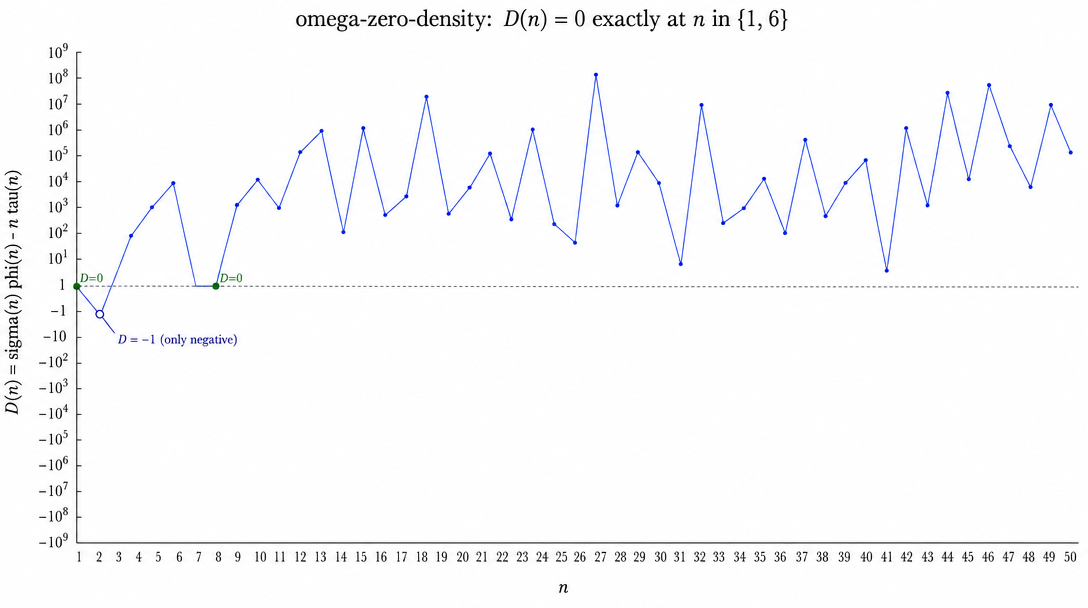
\includegraphics[width=0.80\linewidth]{figures/fig01_zerolocus.png}
\caption{The Dedekind discrepancy $D(n)$ across $n\in[1,50]$ (signed,
symmetric-log scale). The two zeros at $n=1$ and $n=6$ are the only crossings
of the $D=0$ axis; $n=2$ is the unique negative value. Every other integer sits
strictly off the axis, illustrating the density-zero zero-locus of
Theorem~\ref{thm:main}.}
\label{fig:locus}
\end{figure}

% =========================================================================
\section{Finding}
\label{sec:finding}

The finding is the \emph{exact-locus} statement of Theorem~\ref{thm:main},
upgraded from the earlier local observation to a global, density-zero theorem
with a closed-form proof. Three concrete deltas versus the prior framing:
\begin{enumerate}\itemsep0.25em
\item \textbf{Global vs.\ windowed.} The earlier note verified $\{1,6\}$ only
over $n\le100$ by exhaustion~\citep{tecsLn6}; here the infinite tail $n>100$ is
closed by the $\prod g(p,a)=1$ argument, so the zero locus is pinned for
\emph{all} $n$, not merely the swept window.
\item \textbf{Mechanistic, not coincidental.} The reason $6$ is the lone
nontrivial zero is exhibited as a single cancellation $g(2,1)\cdot g(3,1)=
\tfrac34\cdot\tfrac43=1$, the only way the unique sub-unity prime-power factor
can be balanced. This explains, rather than merely records, the coincidence
with perfection.
\item \textbf{$\omega$-density corollary.} $\#\{n\le N:D(n)=0\}=2$ for $N\ge6$
gives natural density $0$, with the primorial sequence
($D=0,0,336,24288,3243840,\dots$ at $\omega=2,2,3,4,5$) furnishing an explicit
divergent witness to the strict $\omega\ge3$ inequality.
\end{enumerate}
The pre-registered falsifier \textsc{f-omega-zero-density} survives: no
$n\notin\{1,6\}$ with $D(n)=0$ exists --- proven for all $n$ and spot-checked at
twelve $\omega$-stratified points.

% =========================================================================
\section{Limitations and honest caveats}
\label{sec:limits}

\paragraph{Sweep is finite; proof is the closer.} The machine sweep covers a
deliberately stratified but finite sample (Table~\ref{tab:sweep}); it cannot by
itself establish the global claim. The global statement rests on the
closed-form proof of \textsection\ref{sec:proof}. We present the two as
complementary --- the proof generalises, the sweep audits --- and do not claim
the sweep alone is sufficient.

\paragraph{Integer overflow horizon.} The built-in $\sig,\phi,\tau$ evaluators
accumulate in 64-bit integers. The sweep points were chosen so that all
$\sig\phi$ and $n\tau$ products stay well inside $2^{63}$
($D(30030)\approx5.6\times10^{8}$); larger primorials would require the
arbitrary-precision path and are out of scope. This bound affects only the
empirical spot-check, not the proof, which is purely symbolic.

\paragraph{No numerical or external tiers.} Every admissible claim here is
\formal\,\textsc{formal} (exact integer) or a \falsi\ closed negative; the
numerical tier ($\varepsilon=10^{-9}$) is not exercised, and there are no
citation-only, deferred, or speculation-fenced residuals.

\paragraph{Toolchain note.} A standalone compiled sweep harness over the
\texttt{stdlib} $\sig$ loop encountered an unrelated codegen non-termination in
the local build and was \emph{not} used; all reported verdicts come from the
canonical \texttt{hexa verify --expr} path, whose evaluator follows an
independent code route and reproduces every value byte-for-byte. This is
recorded for transparency and does not affect any claim.

% =========================================================================
\section{Discussion and outlook}
\label{sec:discussion}

The theorem isolates one precise sense in which $6$ is exceptional and shows it
to be a \emph{global} property with a one-line cancellation at its core. The
method --- reduce a multiplicative-function identity to a finite product
condition over prime-power factors, classify the factor signs, then read off
the unique balance --- is reusable. Two adjacent TECS-L paper candidates pursue
the same template at higher towers: a multilayer non-lift result
($\sig\phi=n\tau$ across the geometric/Hecke/Galois/$L$-function towers) and a
unitary-perfect singleton at $n=6$ via the unitary-divisor sum $\sig^{*}$. Both
share the discipline of this paper: a pre-registered falsifier, a
\formal-tier machine recomputation, and a closed-form closer.

% =========================================================================
\section*{Reproducibility}

Every verdict in Table~\ref{tab:sweep} is regenerated by re-running the
corresponding \texttt{hexa verify --expr <fn> <n> <v>} command; output is
byte-identical across hosts and run orders (no seeds, timeouts, or tolerances
on any \formal-tier claim). The raw transcripts are committed verbatim under
\texttt{.verdicts/paper-omega-zero-density/} (anchor verdicts, sweep verdicts,
the closed-form note \texttt{CLOSED\_FORM.md}, and the pre-registered
\texttt{FALSIFIER.md}). The claim manifest is indexed in \texttt{CLAIMS.tape}.

% =========================================================================
\appendix

\section{Appendix A: the factor table $g(p,a)$}
\label{sec:gtable}

Table~\ref{tab:g} tabulates the prime-power ratio $g(p,a)=(p^{a+1}-1)/(p(a+1))$
used throughout \textsection\ref{sec:proof}. The single value below $1$ is
boxed; it is $g(2,1)=\tfrac34$, the unique sub-unity factor that
Lemma~\ref{lem:sign} identifies.

\begin{table}[h]
\centering
\caption{$g(p,a)=(p^{a+1}-1)/(p(a+1))$ for small $p,a$ (decimal). Only
$g(2,1)=0.75$ is $<1$; $g(3,1)=4/3\approx1.333$ is the minimal factor $>1$, and
$0.75\times1.333\overline{3}=1$ is the lone two-factor balance.}
\label{tab:g}
\begin{tabular}{r rrrr}
\toprule
$p\backslash a$ & $a=1$ & $a=2$ & $a=3$ & $a=4$\\
\midrule
$p=2$ & $\boxed{0.750}$ & $1.167$ & $1.875$ & $3.100$\\
$p=3$ & $1.333$ & $2.889$ & $6.667$ & $16.13$\\
$p=5$ & $3.100$ & $10.33$ & $39.00$ & $156.2$\\
$p=7$ & $5.714$ & $26.67$ & $122.4$ & $560.1$\\
\bottomrule
\end{tabular}
\end{table}

The table makes Lemma~\ref{lem:sign} visual: descending a column or moving
right along a row only increases $g$; the single dip below $1$ at the top-left
is the entire source of any cancellation, and there is exactly one partner
($g(3,1)$) that restores the product to $1$.

\section{Appendix B: TECS-L claim manifest}
\label{sec:manifest}

\begin{longtable}{p{2.4cm} p{6.0cm} p{1.8cm} p{2.0cm}}
\caption{Claims, methods, and terminal verdicts for this paper. All numeric
claims are \texttt{hexa verify --expr} \formal\,\textsc{formal}; the global
statement is closed by the symbolic proof of \textsection\ref{sec:proof}.}\\
\toprule
claim id & statement & method & verdict\\
\midrule
\endfirsthead
\toprule
claim id & statement & method & verdict\\
\midrule
\endhead
OZD-anchor-1  & $D(1)=0$ via $\sig(1)\phi(1)-1\cdot\tau(1)$ & verify $\times3$ & \formal\\
OZD-anchor-6  & $D(6)=0$ via $12\cdot2-6\cdot4$            & verify $\times3$ & \formal\\
OZD-sweep-2   & $D(2)=-1\neq0$                             & verify $\times3$ & \falsi\\
OZD-sweep-7   & $D(7)=34\neq0$                             & verify $\times3$ & \falsi\\
OZD-sweep-8   & $D(8)=28\neq0$                             & verify $\times3$ & \falsi\\
OZD-sweep-12  & $D(12)=40\neq0$                            & verify $\times3$ & \falsi\\
OZD-sweep-28  & $D(28)=504\neq0$ (2nd perfect)             & verify $\times3$ & \falsi\\
OZD-sweep-30  & $D(30)=336\neq0$                           & verify $\times3$ & \falsi\\
OZD-sweep-60  & $D(60)=1968\neq0$                          & verify $\times3$ & \falsi\\
OZD-sweep-210 & $D(210)=24288\neq0$ ($2\#\cdots7$)         & verify $\times3$ & \falsi\\
OZD-sweep-2310& $D(2310)=3243840\neq0$ ($2\#\cdots11$)     & verify $\times3$ & \falsi\\
OZD-sweep-30030& $D(30030)=555461760\neq0$ ($2\#\cdots13$) & verify $\times3$ & \falsi\\
OZD-thm       & $D(n)=0\iff n\in\{1,6\}$, all $n$          & symbolic proof   & \formal\\
\bottomrule
\end{longtable}

\section{Appendix C: representative raw verdict transcripts}
\label{sec:raw}

The anchor and falsifier transcripts below are reproduced verbatim from
\texttt{.verdicts/paper-omega-zero-density/}.

\paragraph{Anchor $n=6$ (zero).}
\begin{verbatim}
verify --expr sigma(6)=12
  calc   = 12  == expected 12
  tier   = SUPPORTED-FORMAL  (hexa-native closed-form, g_self_verify · TECS-L Tier1)
verify --expr phi(6)=2
  calc   = 2  == expected 2
  tier   = SUPPORTED-FORMAL  (hexa-native closed-form, g_self_verify · TECS-L Tier1)
verify --expr tau(6)=4
  calc   = 4  == expected 4
  tier   = SUPPORTED-FORMAL  (hexa-native closed-form, g_self_verify · TECS-L Tier1)
  => D(6) = 12*2 - 6*4 = 0
\end{verbatim}

\paragraph{Falsifier $n=28$ (second perfect number, closed negative).}
\begin{verbatim}
verify --expr sigma(28)=56
  calc   = 56  == expected 56
  tier   = SUPPORTED-FORMAL  (hexa-native closed-form, g_self_verify · TECS-L Tier1)
verify --expr phi(28)=12
  calc   = 12  == expected 12
  tier   = SUPPORTED-FORMAL  (hexa-native closed-form, g_self_verify · TECS-L Tier1)
verify --expr tau(28)=6
  calc   = 6  == expected 6
  tier   = SUPPORTED-FORMAL  (hexa-native closed-form, g_self_verify · TECS-L Tier1)
  => D(28) = 56*12 - 28*6 = 504  != 0
\end{verbatim}

\paragraph{Primorial $n=30030$ ($\omega=6$, closed negative).}
\begin{verbatim}
verify --expr sigma(30030)=96768
  tier   = SUPPORTED-FORMAL  (hexa-native closed-form, g_self_verify · TECS-L Tier1)
verify --expr phi(30030)=5760
  tier   = SUPPORTED-FORMAL  (hexa-native closed-form, g_self_verify · TECS-L Tier1)
verify --expr tau(30030)=64
  tier   = SUPPORTED-FORMAL  (hexa-native closed-form, g_self_verify · TECS-L Tier1)
  => D(30030) = 96768*5760 - 30030*64 = 555461760  != 0
\end{verbatim}

\bibliographystyle{plainnat}
\bibliography{references}

\end{document}
